Unter Landwirtschaft zählen jedoch nicht nur klassische wie Äcker, Maisfelder, Getreidefelder, sondern unter anderem auch Gewächshäuser. Auch in Gewächshäusern gibt es viele Aufgaben, welche durch Sensoren ersetzt, bzw. sogar verbessert werden können.\\
Hier gibt es bereits ein bekanntes Beispiel aus der Heimbeet-Szene:\\

\begin{figure}[h]
	\centering
	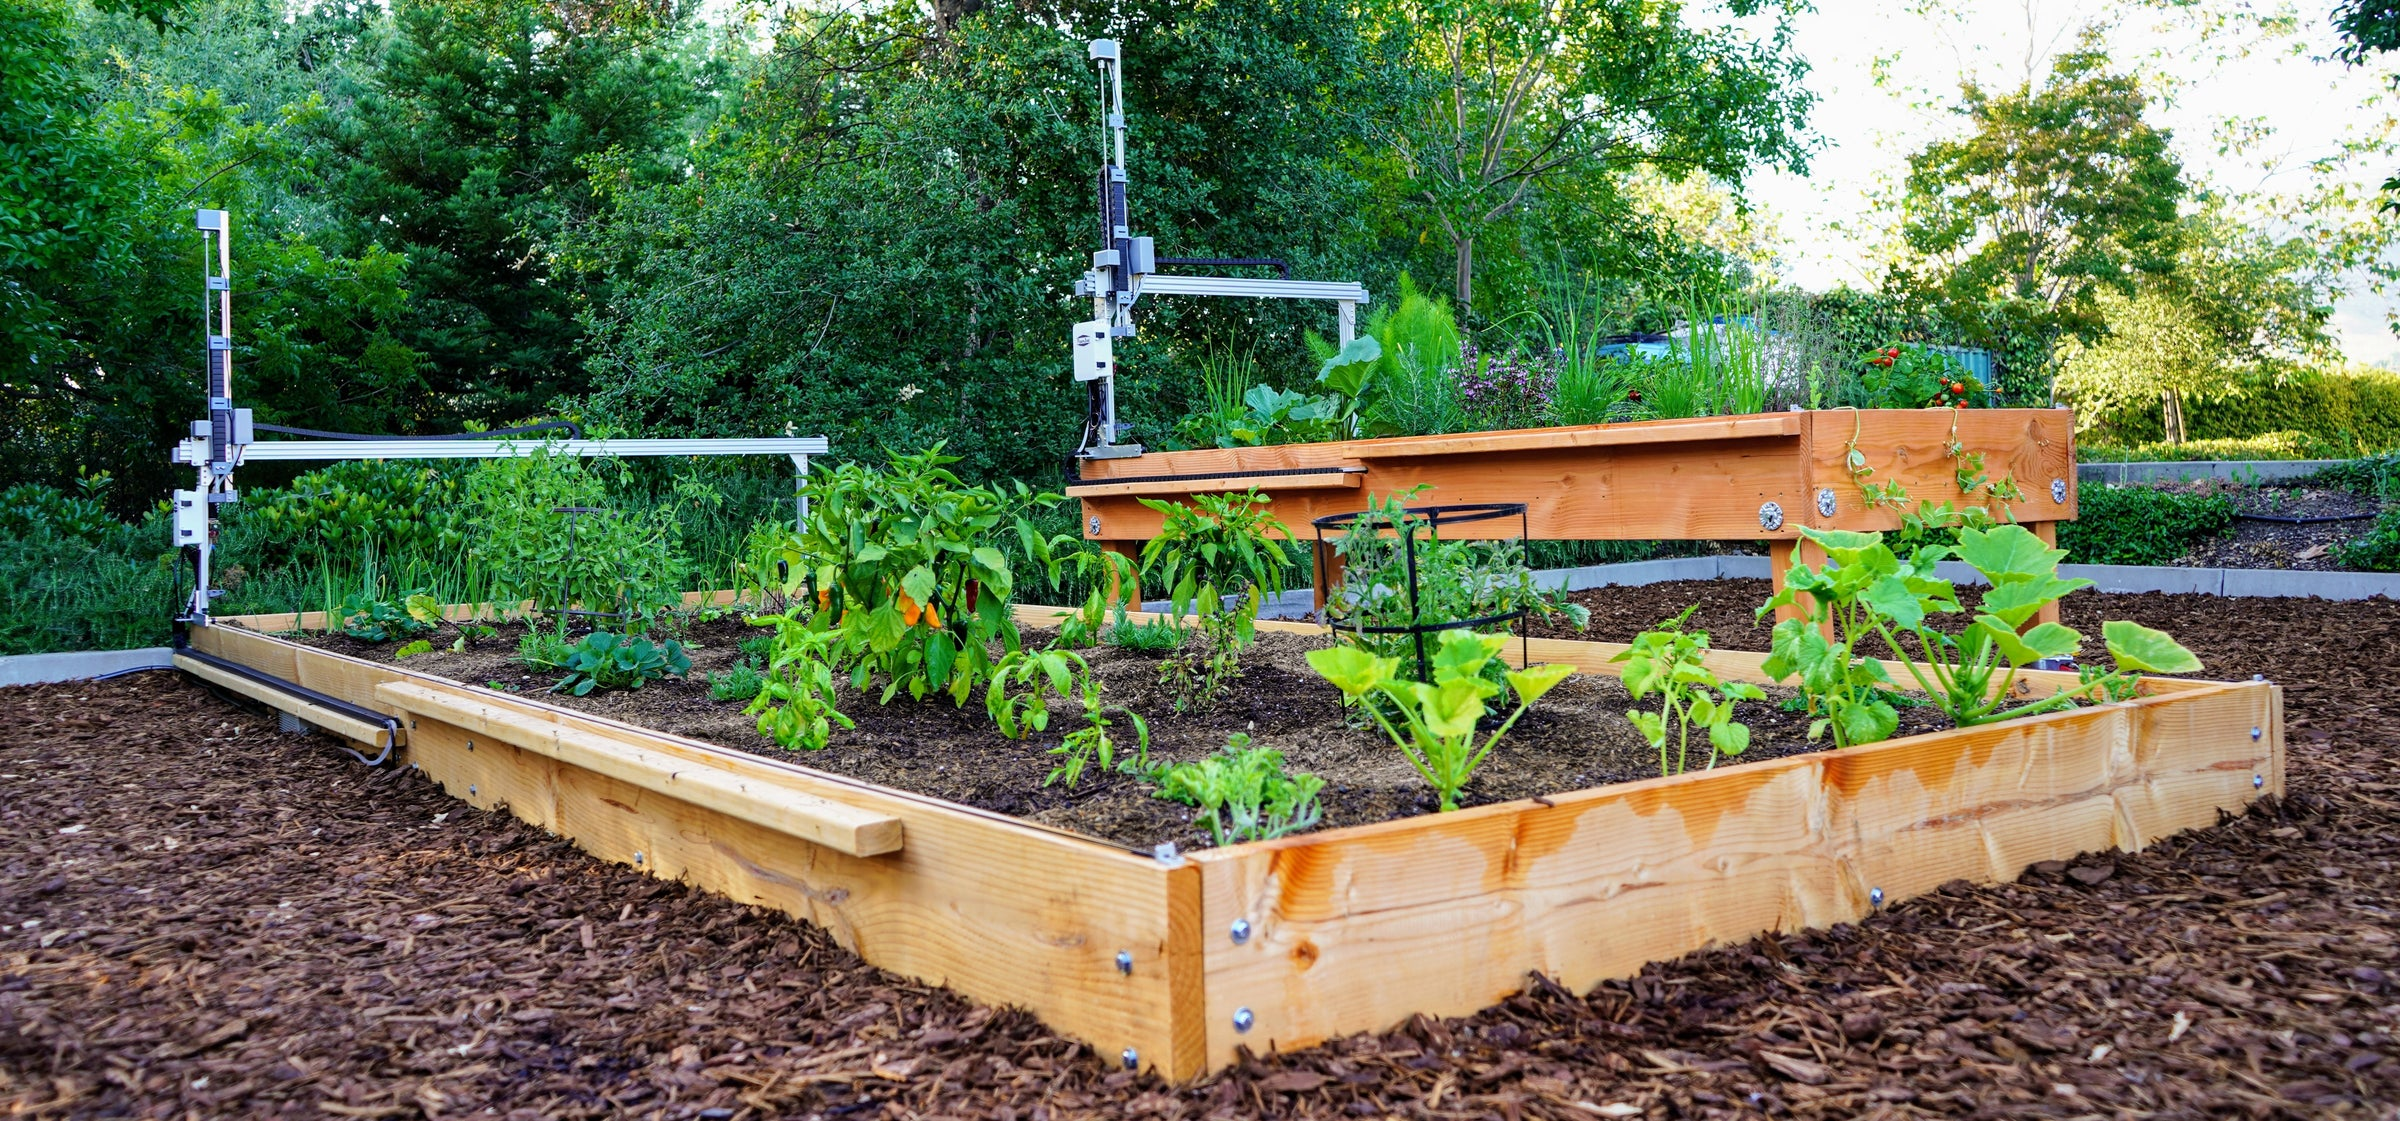
\includegraphics[width=0.5\textwidth]{bilder/farmbot.png}
	\caption[Farmbot]{Farmbot}
	\label{fig:farmbot}
\end{figure}

Der Farmbot ist ein Schienensystem, was von der Mechanik stark an einen 3D-Drucker erinnert. Verkauft wird hierbei von dem Unternehmen nur die Hardware, sprich Schienen, Motoren, Adapter, Verkabelung und ein Raspberry Pi für die Software.\\
Die Software ist open-source, also frei im Internet für alle zugänglich, was mehrere Vorteile mit sich bringt:\\
Die Software wird von jedem User gedownloaded und eventuell umgeschrieben. Das bedeutet die Software wird kontinuierlich Probe gelesen. Außerdem können User die Software verändern und anpassen, etwaige Fehler beheben oder Performance-Verbesserungen vornehmen.